\section{Dynamic Power Reactor}
\label{sec:dpr_method}

The \gls{nrc} publishes a daily Power Reactor Status report for each reactor
under its jurisdiction \cite{nrc_power_2025}. These reports contain, amongst
other things, the percentage of the total power at which the operators
say the reactor operated. This reflects the reality that reactors do not operate at their total power capacity at all times, i.e., their capacity factor is not 1. Fuel cycle simulators can use the effective capacity factor to tell their model how much power to output over time, or they can use data over time to reflect real or imagined fluctuations. The \cycamore reactor assumes that the power is constant, and so, in the case of a fuel cycle simulation containing a small number of reactors or a full-fleet simulation over a short time, the power predicted by the \cycamore reactor and reality can diverge.

Section \ref{sec:transition_scenarios} describes one method of using energy demand to determine the number of reactors to deploy in the future, and such methods can be improved by incorporating realistic power fluctuations. If the reactors are producing more power in the simulation than they would in real life, the simulation will underestimate the number of reactors needed to meet the demand. Additionally, it will not be able to accurately reproduce historical data on the power availability from the fleet of reactors. Figure \ref{fig:pp_full} shows real data from and a \cycamore representation of the single reactor operating at the \gls{clinton}, with a reference unit power (i.e., net power) of 1062 MWe according to the \gls{iaea} \gls{pris} database \cite{IAEA_PRIS}, and compare it to the results from the \cycamore reactor modeled over the same time frame. This figure excludes the startup of the \cycamore reactor to ensure that it was operating on the same schedule as the data from the \gls{nrc} suggest the reactor was operating on from the start of 2021 through the end of 2024.

\begin{figure}[H]
  \centering
  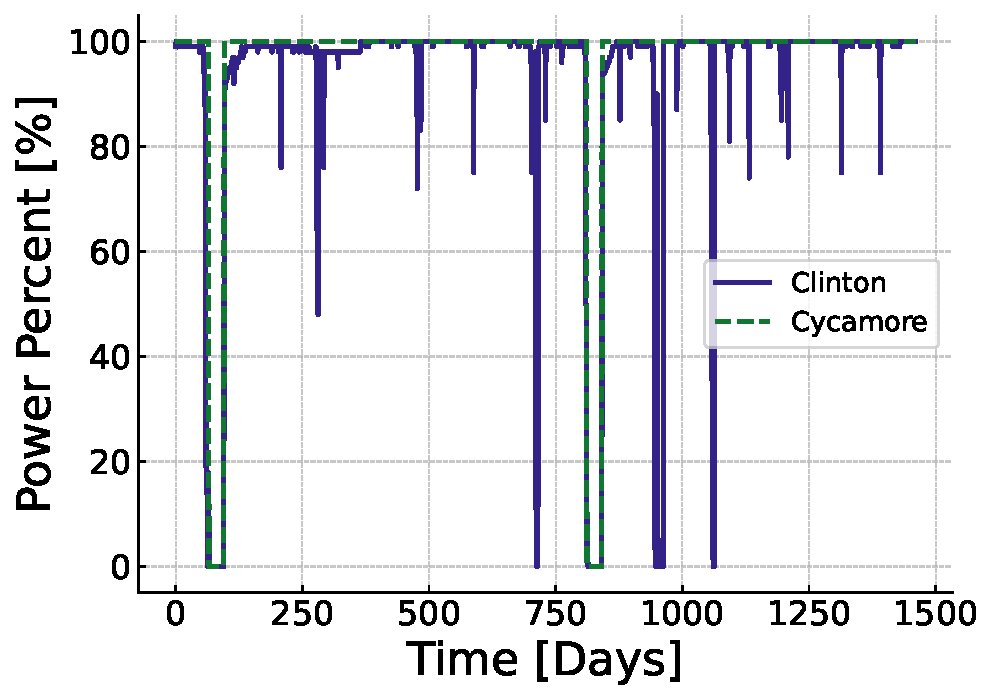
\includegraphics[width=0.7\linewidth]{images/power_reactor/power_percent_clinton_fake.pdf}
  \caption{\gls{clinton} reactor daily capacity factor 2021-2024.}
  \label{fig:pp_full}
\end{figure}

A simple numerical integration reveals that the total energy capacity of both reactors differs by just under 51 GWe with a percent difference of 3.52\%; however, the two scenarios in Figure \ref{fig:pp_full} were not equal on 908 days, or 62.2\%, of the 1460-day simulation. This thesis introduces the \gls{dpr} to mirror this variability in power of an operating reactor to capture these temporal fluctuations. \gls{dpr} functions the same way as the \cycamore reactor, except the user can input the percentage of the total capacity the reactor is outputting at any given time step.

% \begin{figure}[H]
%   \centering
%   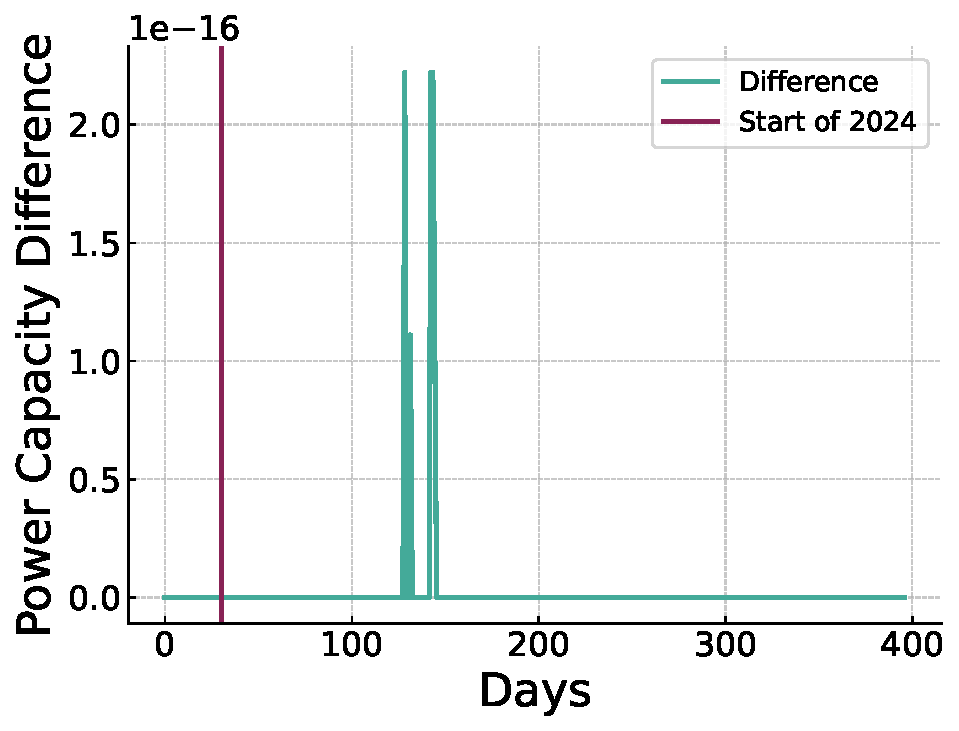
\includegraphics[width=0.7\linewidth]{images/power_reactor/dpr_diff.pdf}
%   \caption{Difference in daily capacity factor between \gls{clinton} and \gls{dpr}'s Clinton.}
%   \label{fig:dpr_clinton_diff}
% \end{figure}


Narrowing the scope of this study to 2024, this thesis uses \gls{dpr} to replicate the capacity factor fluctuations of \gls{clinton}. The maximum difference between the reported values from the \gls{nrc} \cite{nrc_power_2025} and the results from the \cyclus simulation is $2.22 \times 10^{-16}$ GWe, which is explainable by floating point error in calculations as this value matches a double point machine epsilon value. Figure \ref{fig:dpr_cycamore_power} compares \gls{dpr} to the \cycamore reactor. As the reactors are assumed to start operations before 2024, a buffer month in which the reactors receive fuel allows these results to align with reality. The vertical line indicates when 2024 begins, allowing Figure \ref{fig:dpr_cycamore_power} to compare the \gls{nrc} data with results from \cyclus. Although the \cycamore reactor was able to reproduce the \gls{clinton} reactor's power output around refueling outages, the \gls{dpr} is able to reproduce all of the fluctuations in power output even in years that did not have a refueling outage.

\begin{figure}[H]
  \centering
  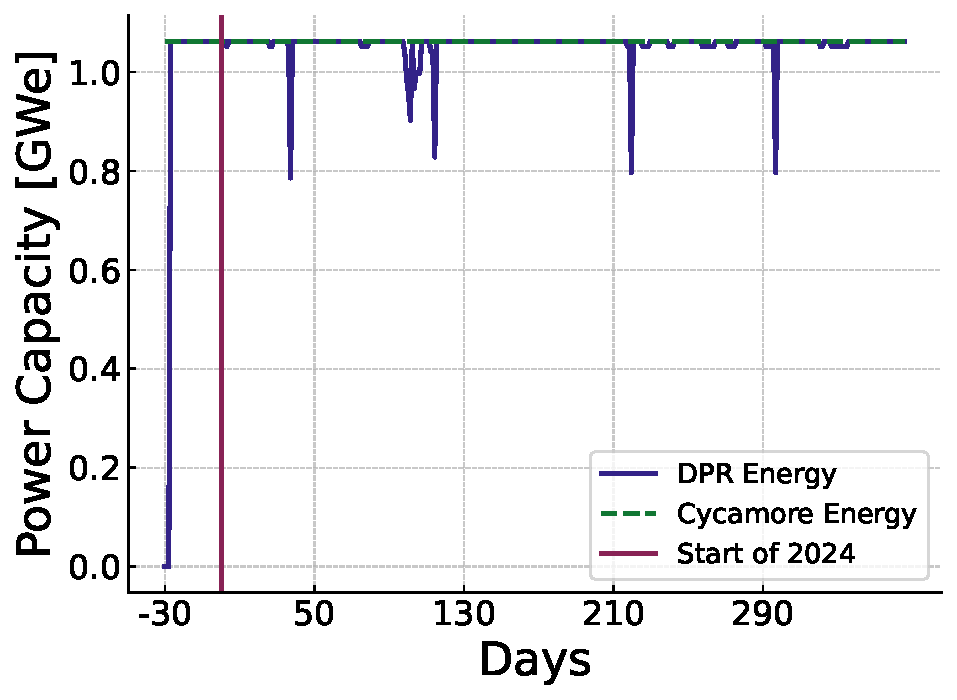
\includegraphics[width=0.7\linewidth]{images/power_reactor/dpr_cycamore_energy.pdf}
  \caption{2024 capacity factor of the \cycamore reactor and \gls{dpr}.}
  \label{fig:dpr_cycamore_power}
\end{figure}

